\chapter{Background}
\section{Turing Machine}
\subsection{Introduction to Turing Machines}
A \emph{Turing Machine} (TM) is a collection $(Q, \Sigma, \delta, q_0)$, where:
\begin{itemize}
    \item $Q$ is a set of \emph{states}, including the \emph{accept state} $A$ and the \emph{reject state} $R$;
    \item $\Sigma$ is a set of \emph{letters}, called the \emph{alphabet}, which does not include the \texttt{blank} symbol;
    \item $\delta \colon Q \setminus \{A, R\} \times \Sigma^+ \to Q \times \Sigma^+ \times \{\texttt{left}, \texttt{right}\}$, where $\Sigma^+ = \Sigma \cup \{\texttt{blank}\}$, is the \emph{transition function}; and
    \item $q_0 \in Q$ is the \emph{starting state}.
\end{itemize}
Although based on Turing's work on \citet{turing1936computable}, this definition, along with others in this section, have been adapted from \citet{hopcroft2001automata}.

\begin{figure}[htb]
    \centering
    \begin{subfigure}{0.45\textwidth}
        \centering
        \begin{tikzpicture}
            \node[state, accepting] (q0) at (0, 0) {$q_0$};
            \node[state] (q1) at (2.5, 0) {$q_1$};
            \node[state, fill=green, opacity=0.6] (A) at (5, -1) {$A$};
            \node[state, fill=red, opacity=0.6] (R) at (5, 1) {$R$};
    
            \draw[->] (q0) edge[loop above] node[text width=1.5cm, align=center] {$0 \to 0, R$ $1 \to 1, R$} (q0);
            \draw[->] (q0) -- node[above] {$\# \to \#, L$} (q1);
            \draw[->] (q1) -- node[below, rotate=-20] {$0 \to \#, L$} (A);
            \draw[->] (q1) -- node[above, rotate=20, text width=1.5cm, align=center] {$1 \to 1, L$ $\# \to \#, L$} (R);
        \end{tikzpicture}
        \caption{Full notation}
    \end{subfigure}
    \hfill
    \begin{subfigure}{0.45\textwidth}
        \centering
        \begin{tikzpicture}
            \node[state, accepting] (q0) at (0, 0) {$q_0$};
            \node[state] (q1) at (2.5, 0) {$q_1$};
            \node[state, fill=green, opacity=0.6] (A) at (5, -1) {$A$};
            \node[state, fill=red, opacity=0.6] (R) at (5, 1) {$R$};
    
            \draw[->] (q0) edge[loop above] node {$0|1, R$} (q0);
            \draw[->] (q0) -- node[above] {$\#, L$} (q1);
            \draw[->] (q1) -- node[below, rotate=-20] {$0 \to \#, L$} (A);
            \draw[->] (q1) -- node[above, rotate=20] {$1|\#, L$} (R);
        \end{tikzpicture}
        \caption{Shorthand notation}
    \end{subfigure}
    \caption{A FSM representation of a TM that accepts binary numbers divisible by 2.}
    \label{fig:tm_isDiv2}
\end{figure}

We can \textit{represent} a TM as a \emph{finite state machine} (FSM). This is a directed graph, with vertices as states and edges as transitions. An example is given in Figure \ref{fig:tm_isDiv2}. In this case, the alphabet $\Sigma = \{0, 1\}$. The \texttt{blank} symbol is denoted by $\#$. The initial state is denoted by $q_0$; the accept state $A$ and the reject state $R$. Every edge corresponds to an evaluation of the transition function $\delta$, e.g. $\delta(q_1, 0) = (A, \texttt{blank}, \texttt{left})$. 

The figure presents two ways of representing a FSM- subfigure (a) shows the transitions explicitly, whereas subfigure (b) is less explicit:
\begin{itemize}
    \item It hides the transition value if it is not getting changed ($\#, L$ instead of $\# \to \#, L$). 
    \item It also combines the letters whose transition values are not being changed and have the same transition state and direction ($0|1, L$ instead of $0, L$ and $1, L$). 
\end{itemize}
We will make use of the shorthand notation.

FSMs are considered a \emph{representation} of a TM. This word has a very specific meaning, in that there is a bijection between FSMs (of the format given above) and TMs. Moreover, there is a `simple' algorithm that allows us to convert a FSM to a TM, and vice versa.

\subsection{Executing a TM on a tape}
Let $\Sigma$ be an alphabet. A \emph{tape} $T$ on $\Sigma$ is a function $T\colon \mathbb{Z} \to \Sigma^+$. That is, the tape has infinite entries in both directions. Moreover, each tape entry contains a value from the alphabet, or the \texttt{blank} symbol. 

\begin{figure}[htb]
    \centering
    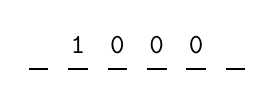
\begin{tikzpicture}
        \foreach \x[count=\i] in {, 1, 0, 0, 0, } {
            \draw[thick] (\i*0.5-0.25, 0) -- (\i*0.5, 0);
            \node at (\i*0.5-0.125, 0.3) {\texttt{\x}};
        }
    \end{tikzpicture}
    \caption{A TM tape on $\{0, 1\}$.}
    \label{fig:tape_example}
\end{figure}
We can specify a tape using a figure. For instance, let $\Sigma = \{0, 1\}$, and let $T$ be the tape on $\Sigma$ given as follows:
\[T(x) = \begin{cases}
    0 & x \in \{0, 2, 3\} \\
    1 & x \in \{1\} \\
    \texttt{blank} & \text{otherwise}.
\end{cases}\]
Then, Figure \ref{fig:tape_example} illustrates the tape $T$. We will assume that the first non-blank value is at index 0.

We can execute a TM on a tape. Let $M$ be a TM with alphabet $\Sigma$, and let $T$ be a tape on $\Sigma$. We execute $M$ on $T$ inductively, as follows:
\begin{itemize}
    \item At any point during execution, we maintain 3 objects: a tape on $\Sigma$; a (current) state in $M$; and an index in the tape (called the \emph{tapehead index}).  

    \item At the start, the tape is $T$; the tapehead index is $0$; and the current state is the initial state $q_0$. 
    
    \item At some point during the execution, assume that we have the tape $S$, tapehead index $j$, with \emph{tapehead value} $T(j) = t$, and a non-terminating state $q$ (i.e. not $A$ or $R$). Denote $\delta(q, t) = (q', t', \texttt{dir})$. Then, 
    \begin{itemize}
        \item the next state is $q'$;
        \item the next tape is $S'$, where
        \[S'(x) = \begin{cases}
            t' & x = i \\
            S(x) & \text{otherwise};
        \end{cases}\]
        and
        \item the next tapehead index is $j'$, where
        \[j' = \begin{cases}
            j+1 & \texttt{dir} = \texttt{right} \\
            j-1 & \texttt{dir} = \texttt{left}.
        \end{cases}\]
    \end{itemize}
    If the state $q'$ is not a terminating state, then the execution continues with these 3 objects. Otherwise, execution is terminated with the terminating state $q'$.
\end{itemize}

\begin{figure}[htb]
    \centering
    \begin{subfigure}{0.4\textwidth}
        \centering
        \begin{tikzpicture}
            \foreach \x[count=\i] in {, 1, 0, 0, 0, } {
                \draw[thick] (\i*0.5-0.25, 0) -- (\i*0.5, 0);
                \node at (\i*0.5-0.125, 0.3) {\texttt{\x}};
            }
            \draw[->] (2.875, -0.5) -- (2.875, -0.1);
        \end{tikzpicture}
        \caption{}
    \end{subfigure}
    \begin{subfigure}{0.4\textwidth}
        \centering
        \begin{tikzpicture}
            \foreach \x[count=\i] in {, 1, 0, 0, , } {
                \draw[thick] (\i*0.5-0.25, 0) -- (\i*0.5, 0);
                \node at (\i*0.5-0.125, 0.3) {\texttt{\x}};
            }
            \draw[->] (1.875, -0.5) -- (1.875, -0.1);
        \end{tikzpicture}
        \caption{}
    \end{subfigure}
    \caption{Some of the tape states during execution.}
    \label{fig:tm_tape_execution}
\end{figure}
We illustrate this process with the TM in Figure \ref{fig:tm_isDiv2} with the tape in Figure \ref{fig:tape_example}:
\begin{itemize}
    \item Initially, the tape is the given tape; $q_0$ is the current state; and the tapehead index is $0$, with value $1$.
    
    \item According to the FSM, we have $\delta(q_0, 1) = (q_0, 1, R)$. Hence,
    \begin{itemize}
        \item the tape remains unchanged;
        \item $q_0$ is still the current state; and
        \item and the tapehead index becomes $1$, with value \texttt{0}.
    \end{itemize}
    
    \item The transition for \texttt{0} and \texttt{1} are essentially the same with respect to $q_0$. This means that we keep moving to the right until we end up at a \texttt{blank} symbol. At that point, the state of the tape is given in Figure \ref{fig:tm_tape_execution} (a). The arrow points at the tapehead entry. We are still at the state $q_0$, and the tape has not been altered.
    
    \item Now, since the tapehead value is \texttt{blank}, we move to the left and the current state becomes $q_1$. The tape has still not been changed. The current value is now $0$.
    
    \item We have $\delta(q_1, 0) = (A, \texttt{blank}, L)$. So, 
    \begin{itemize}
        \item the tapehead value changes to from $0$ to blank;
        \item the current state becomes $A$; and
        \item the tapehead pointer move to the left, to index $2$.
    \end{itemize}
    Since $A$ is a terminating state, execution terminates, with result \texttt{accept}. The final tape state is given in Figure \ref{fig:tm_tape_execution} (b).
    
\end{itemize}
So, the TM in Figure \ref{fig:tm_isDiv2} executes as follows:
\begin{itemize}
    \item we use the state $q_0$ to traverse to the first blank symbol (i.e. the end of the string), and then move to the state $q_1$;
    \item at state $q_1$, we accept the string if and only if the current tapehead value is \texttt{0}
\end{itemize}
Hence, this TM accepts binary numbers if and only if they are divisible by 2.

\subsection{TM as a model of computation}
Turing initially proposed TMs as the `correct' model of computation in \citet{turing1936computable}. This result is called the \emph{Church-Turing Thesis}. It is a \textit{thesis} since it is informal in nature; it is just a \textit{belief} that the correct model of computation is the model given by TMs. 

In this paper, Turing also showed that TMs and $\lambda$-calculus are equivalent. Hence, it follows that $\lambda$-calculus is also the correct model of computation. There have been many other models of computations proposed, such as general recursive functions. It is widely regarded that TMs (and all the equivalent models) specify the correct model of computation. This is because many of the originally proposed models of computation turned out to be equivalent \citep{copeland2004essential}.

\subsection{Learning Automata Theory}
Students tend to struggle learning automata theory, which includes TMs. This has been associated with the theoretical and mathematical nature of the topic \citep{wermelinger2005prolog}. As such, students claim that the lectures covering the topic are boring, monotonous and unengaging \citep{pillay2010learning}. 

This is also visible in student performance. In particular, when students were taught automata theory using the pen-and-paper method, i.e. by drawing FSMs, many tend to give the wrong answer \citep{rodger2006jflap}. \citet{rodger2009increasing} mentions that this is likely because they find it tedious to check the correctness of the FSM.

There have been many attempts made to improve student engagement in automata theory. 
\begin{itemize}
    \item There are visualisation tools that allow students to construct automata and then test simulate execution on a string. One of these tools is JFLAP, which has support for TMs \citep{rodger2006jflap}. \citet{rodger2009increasing} found that making use of this tool helped boost student engagement and performed better overall than those who had not made use of the tool. In general, algorithm animators have generally proven to be quite effective in supplementing courses \citep{stasko1998empirically}.
    
    \item In \citet{tecson2018tutoring}, a website was used by students to learn automata theory. Many students enjoyed this approach since it was flexible and allowed them to learn at their pace. Moreover, it offered visualisations (i.e. FSMs) and allowed the students to execute the FSM on a tape.
    
    \item In \citet{wermelinger2005prolog}, a package was created in Prolog to allow students to construct FSMs programmatically. The FSMs can be simulated to test for the language they accept. This was created to bridge the gap between programming languages and automata theory, and it was hoped that the package would improve student engagement and performance.
\end{itemize} 

Although there are many other proposals in literature, most tend to be similar visualisation techniques \citep{zingaro2008another}. Novel ideas are necessary to understand further how to keep students motivated in learning automata theory. 

\section{Parser}
A \emph{compiler} is a program that takes source code in a programming language (PL) and translates it into a program in another PL. An \emph{interpreter} is a program that takes source code in a programming language and executes it directly. During the process, the compiler and the interpreter detect errors, such as syntax and type errors.

\begin{figure}[htb]
    \centering
    \begin{subfigure}[b]{0.4\textwidth}
        \centering
        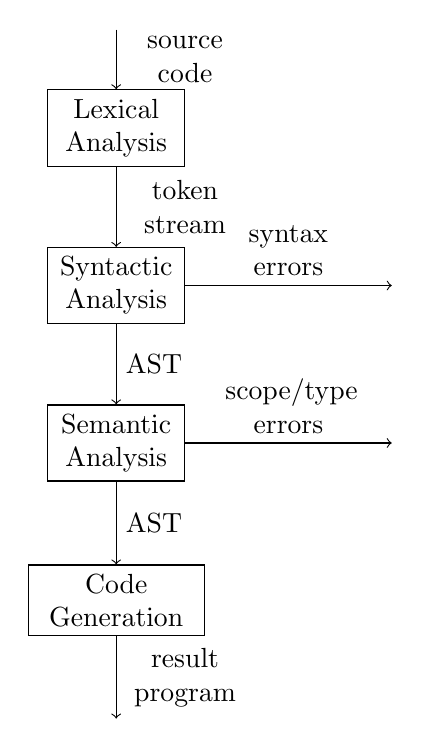
\begin{tikzpicture}
            \node[draw, text width=1.5cm, align=center] (LA) at (0, 0) {Lexical Analysis};
            \node[draw, text width=1.5cm, align=center] (SA) at (0, -2) {Syntactic Analysis};
            \node[draw, text width=1.5cm, align=center] (CA) at (0, -4) {Semantic Analysis};
            \node[draw, text width=2cm, align=center] (CG) at (0, -6) {Code Generation};
            
            \draw[->] (0, 1.25) -- node[right, text width=1.5cm, align=center] {source code} (LA);
            \draw[->] (LA) -- node[right, text width=1.5cm, align=center] {token stream} (SA);
            
            \draw[->] (SA) -- node[above, text width=1.5cm, align=center] {syntax errors} (3.5, -2);
            \draw[->] (SA) -- node[right] {AST} (CA);
            \draw[->] (CA) -- node[above, text width=1.6cm, align=center] {scope/type errors} (3.5, -4);
            
            \draw[->] (CA) -- node[right] {AST} (CG);
            \draw[->] (CG) -- node[right, text width=1.5cm, align=center] {result program} (0, -7.5);
        \end{tikzpicture}
        \caption{Compilation}
    \end{subfigure}
    \hfill
    \begin{subfigure}[b]{0.4\textwidth}
        \centering
        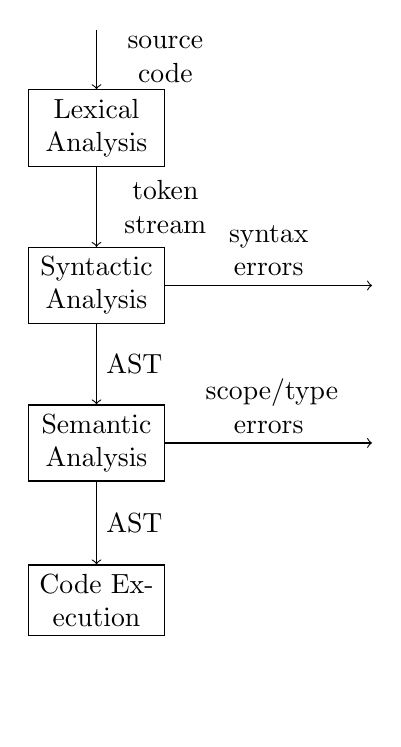
\begin{tikzpicture}
            \node[draw, text width=1.5cm, align=center] (LA) at (0, 0) {Lexical Analysis};
            \node[draw, text width=1.5cm, align=center] (SA) at (0, -2) {Syntactic Analysis};
            \node[draw, text width=1.5cm, align=center] (CA) at (0, -4) {Semantic Analysis};
            \node[draw, text width=1.5cm, align=center] (CG) at (0, -6) {Code Execution};
            
            \draw[->] (0, 1.25) -- node[right, text width=1.5cm, align=center] {source code} (LA);
            \draw[->] (LA) -- node[right, text width=1.5cm, align=center] {token stream} (SA);
            
            \draw[->] (SA) -- node[above, text width=1.5cm, align=center] {syntax errors} (3.5, -2);
            \draw[->] (SA) -- node[right] {AST} (CA);
            \draw[->] (CA) -- node[above, text width=1.6cm, align=center] {scope/type errors} (3.5, -4);
            
            \draw[->] (CA) -- node[right] {AST} (CG);
            \draw[white] (CG) -- (0, -7.5);
        \end{tikzpicture}
        \caption{Interpretation}
    \end{subfigure}
    \caption{The data flow during (a) compilation and (b) interpretation.}
    \label{fig:compilation_and_interpretation}
\end{figure}

We will now consider the different phases of the compilation and interpretation process. This is summarised in Figure \ref{fig:compilation_and_interpretation}. This figure, along with most of the content in this section, has been adapted from \citet{aho2007compilers}. As we can see, many of the phases are the same between the two processes.

\subsection{Lexical Analysis}    
The first stage of compilation and interpretation is \emph{lexical analysis}. In this stage, the source code is enriched to make it ready for parsing. In particular, we generate a stream of source code, which reads the program word by word. Then, it produces a stream of \emph{tokens}. A token is a word in source code along with a label. For instance, consider the mathematical expression \texttt{1 + 2}. We can convert this expression into 3 tokens: \texttt{(1, NUM)}, \texttt{(+, PLUS)} and \texttt{(2, NUM)}. 

\subsection{Syntactic Analysis}

Next, we try to parse the token stream into an \emph{abstract syntax tree} (AST). If there are syntax errors present in the program, then it is not possible to construct an AST. This will be detected during the process, at which point we can throw a syntax error.

\begin{figure}[htb]
    \centering
    \begin{tikzpicture}[
        level distance=1.2cm,
        level 1/.style={sibling distance=4cm},
        level 2/.style={sibling distance=2cm},
    ]
        \node[ellipse, draw] {TIMES}
        child {
            node[ellipse, draw] {PLUS}
            child {
                node[draw] {\texttt{1}}
            }
            child {
                node[draw] {\texttt{2}}
            }
        }
        child {
            node[ellipse, draw] {PLUS}
            child {
                node[draw] {\texttt{3}}
            }
            child {
                node[draw] {\texttt{4}}
            }
        };
    \end{tikzpicture}
    \caption{The AST for the expression \texttt{(1 + 2) * (3 + 4)}}
    \label{fig:AST_example}
\end{figure}

An AST presents the program as a tree. Typically, the internal nodes specify operations, while the leaves give their arguments. The AST for the expression \texttt{(1 + 2) * (3 + 4)} is given in Figure \ref{fig:AST_example}.

There are many ways to parse the stream of tokens. A common method is \emph{recursive-descent parsing}. Here, we have a parser function for each construct in the language, such as a \textit{program}, an \textit{if} command, an \textit{expression}, etc. We typically look at the next token value and choose a function. 

One way of performing recursive-descent parsing is by \emph{top-down parsing}. In this case, we produce the parent node of the AST and then generate its children. 

The simplest form of recursive-descent parsing is called \emph{predictive parsing}. This applies when the next token determines what structure it is to be parsed. For instance, if we see the token \texttt{if}, then we know we are parsing an \textit{if} command.

\subsection{Semantic Analysis}
Now, we traverse the AST and check that there are no errors in the source code. Typically, there are 2 types of things to check in this stage- \emph{type errors} and \emph{scope errors}. 

In type errors, we check whether the AST has some type mismatch, e.g. \texttt{1 + true}. We can detect this by keeping track of the types of the identifiers and see if they are legal.

In scope errors, we ensure that all the identifiers present in code are defined. To do so, we need to keep track of all the variables that are in scope. In terms of functions, there is a design choice here- we can have all functions in scope from the start, or add them to scope as they are encountered. Another thing to consider is recursion- to allow recursion, the function must be in scope as soon as it is declared.

\subsection{Code Generation}
During the final stage of compilation, we convert the AST into code in the target language. In particular, we traverse the tree and convert each phrase from the source language to the target. The actual structure of this process depends on the target language.

\subsection{Code Execution}
During the final stage of interpretation, we execute the code. This is done by traversing the AST, and then executing each block of code. Like with code generation, this process is dictated by the structure of the source language.
